\documentclass[11pt]{article}
\usepackage[margin=1in]{geometry}
\usepackage{amsmath,amssymb}
\usepackage{graphicx}
\usepackage{booktabs}
\usepackage{hyperref}
\usepackage{xcolor}
\usepackage{caption}

\title{The Roughness Exercise: Calibrating the Optimal ESN--A2 Architecture\\
Directly to Real Assets' and Indices' Own Roughness}
\author{Companion note to the ESN A2-981003 market-data hyperparameter search}
\date{August 14, 2026}

\begin{document}
\maketitle

\begin{abstract}
The companion note (\emph{ESN--A2 Hyperparameter Search: Full-Parameter Grid with
Smooth Surrogate Statistics, Optimised via Bounded Levenberg--Marquardt}) finds an
optimal architecture, $N_r=22,N_z=29$, by grid-averaging the calibrated parameter
vector $p$ and fitting 5 real S\&P~500 assets simultaneously. This note asks a
different, more targeted question: \textbf{fixing that architecture}, can 4 of the
12 entries of $p$ that govern the reservoir's own roughness -- $H$,
\texttt{rough\_scale}, $\lambda_{lo}$, and $\lambda_{hi}$ -- be calibrated, per
asset, to reproduce that asset's own real log-volatility roughness, measured
directly via the standard moment-scaling (structure-function) Hurst estimator from
the rough-volatility literature?

\textbf{9 real assets} are examined: 6 individual stocks (\texttt{LH}, \texttt{SPGI},
\texttt{DOV}, \texttt{F}, \texttt{UDR}, \texttt{SO}) and 3 major U.S.\ market
indices (\texttt{SP500}, \texttt{RUSSELL2000}, \texttt{NASDAQ100}). Each asset's
own real, bias-corrected moment-based Hurst exponent is used as a direct
calibration target -- not the companion note's 11-term aggregate stylised-fact
score -- and the 4 parameters are optimised, per asset, to close the gap between
that target and the ESN's own simulated roughness, with the optimisation objective
strengthened (more simulated paths per evaluation, multiple starting points) until
genuine convergence is confirmed against an independent, long simulated path and a
60-replicate empirical distribution.

\textbf{The result: every one of the 9 assets' calibrated ESN reproduces that
asset's own real Hurst exponent to within 1 empirical standard deviation}
($|z|<1$ for all 9; mean $|z|=0.44$; \texttt{DOV} and \texttt{SO} essentially
exact, $|z|<0.1$) -- 6 individual stocks and 3 diversified market indices alike,
despite the indices' real roughness sitting on the \emph{opposite} side of the
ESN's own achievable range from the stocks' (real stocks are rougher than their
calibrated ESN; real indices are smoother). The same fixed architecture, restricted
to these 4 roughness-related free parameters, is flexible enough to reproduce the
moment-based Hurst exponent of every asset examined here, once calibrated directly
to that target with an adequately robust optimisation.
\end{abstract}

\tableofcontents

\section{Motivation and set-up}
The main search (companion note, \S1.6) grids all 12 entries of the calibrated
parameter vector $p=(H,\lambda_{lo},\lambda_{hi},a_{lo},a_{hi},\Delta b_0,\text{scale},
\texttt{rough\_scale},\texttt{zr\_lo},\texttt{zr\_hi},m_1,m_2)$ over a wide admissible
range and averages the resulting stylised facts across the grid, fitting all 5
calibration assets \emph{simultaneously} via a single 55-entry residual vector. That
procedure answers ``what architecture and averaged $p$-behaviour best explains 5
assets at once'', but does not directly show how well the resulting architecture can
be tuned to \emph{one} asset's own roughness specifically.

This note isolates that question. The 9 architecture hyperparameters
($N_r,N_z$ + 7 shared z-bank hyperparameters) are \textbf{fixed} at the companion
note's optimum:
\begin{center}
\begin{tabular}{lr}
\toprule
Hyperparameter & Value \\
\midrule
$N_r$ & 22 \\
$N_z$ & 29 \\
\texttt{z\_strength} & 0.2714 \\
\texttt{even\_strength} & 3.1843 \\
\texttt{linear\_strength} & 0.1820 \\
\texttt{gamma\_norm} & 1.3081 \\
\texttt{local\_z\_strength} & 0.0608 \\
\texttt{zz\_scale} & 0.0312 \\
\texttt{sign\_prob\_neg} & 0.2228 \\
\bottomrule
\end{tabular}
\end{center}
Of the 12 entries of $p$, \textbf{4 roughness-related entries are calibrated, per
asset}: $H$, \texttt{rough\_scale}, $\lambda_{lo}$, and $\lambda_{hi}$. The
remaining 8 are held fixed at reasonable centre values (not re-optimised, not
gridded):
\begin{center}
\begin{tabular}{lr|lr}
\toprule
Entry & Value & Entry & Value \\
\midrule
$a_{lo}$ & $1/400$ & \texttt{zr\_lo} & 0.055 \\
$a_{hi}$ & $1/7$ & \texttt{zr\_hi} & 0.25 \\
$\Delta b_0$ & 0.0 & $m_1$ & 0.0 \\
\text{scale} & 1.0 & $m_2$ & 0.0 \\
\bottomrule
\end{tabular}
\end{center}
$\lambda_{lo}$ and $\lambda_{hi}$ set the reservoir's slowest and fastest
Ornstein--Uhlenbeck rates -- together with $H$ and \texttt{rough\_scale}, they
directly govern the reservoir's own achievable roughness (\S\ref{sec:calibexplain}
explains the mechanism); the other 8 entries shape different aspects of the
simulated path (the nonlinear $z$-bank's own timescales and readout profile, the
quadratic coupling, the drift and scale) and are left fixed so that this note's
results are attributable to the 4 roughness-governing parameters specifically.

\subsection{9 real assets}
The companion note's 5 calibration assets (\texttt{GPC}, \texttt{QCOM}, \texttt{INTC},
\texttt{LUV}, \texttt{NI}) are drawn from the S\&P~500 panel
(\texttt{list\_dics\_SP500\_ohlcvol\_19940101\_filtered.pkl}, 243 tickers) via a fixed
random permutation (seed 11). This note examines \textbf{9 further assets} in total:
\textbf{6 individual stocks} -- 3 continuing that \emph{same} deterministic sequence,
\texttt{LH} (Labcorp Holdings), \texttt{SPGI} (S\&P Global), \texttt{DOV} (Dover
Corp), and 3 more from a separate, independently randomised selection (seed 777),
\texttt{F} (Ford), \texttt{UDR} (UDR Inc.), \texttt{SO} (Southern Company) -- and
\textbf{3 market indices}, \texttt{SP500} (S\&P 500, \texttt{\^{}GSPC}),
\texttt{RUSSELL2000} (Russell 2000, \texttt{\^{}RUT}), and \texttt{NASDAQ100}
(Nasdaq-100, \texttt{\^{}NDX}) -- OHLC index-level data (not a constituent-stock
proxy), covering 1994-01-03 to 2023-11-14 (7,521 trading days; the panel's own
history runs to 2025, so the index history is the shorter of the two but still
substantial). All 9 use the same admissibility rule (full available history,
$\ge5$ of 6 windows usable) as the companion note's own 5.

\section{Explicitly explaining the calibration}
\label{sec:calibexplain}

\subsection{What $H$, \texttt{rough\_scale}, $\lambda_{lo}$, and $\lambda_{hi}$ control in the simulator}
Recall the ESN's pre-activation (companion note \S1.2):
\[
\eta_t = b_0 + \rho_r\,\texttt{rough\_scale}\,(q^\top r_t)
       + \sum_{j=1}^{N_z} w_{j,z}\,z_{j,t} + r_t^\top Q\, r_t,
\]
where $r_t$ is the linear reservoir, built from $N_r$ Ornstein--Uhlenbeck processes
with rates $\lambda_i$ geometrically spaced across $[\lambda_{lo},\lambda_{hi}]$, and
$q_i\propto\lambda_i^{0.5-H}$ is $H$'s own weighting of those modes.
\texttt{rough\_scale} is a pure amplitude knob on the linear channel $q^\top r_t$;
$H$ reshapes how the $N_r$ discrete OU modes are weighted relative to each other;
$\lambda_{lo}$ and $\lambda_{hi}$ set the slowest and fastest timescales the
reservoir includes at all. \textbf{Isolating the linear channel $q^\top r_t$ from
the rest of the simulator (no $z$-bank, no softplus) shows its own moment-based
roughness matches the full simulated log-volatility's to 4 decimal places}: the
$z$-bank contributes negligibly, and the roughness this note calibrates is governed
almost entirely by this one channel and its 4 parameters.

$\lambda_{hi}$ in particular has an outsized, and non-obvious, effect: at a high
$\lambda_{hi}$, the reservoir's fastest mode decorrelates on a sub-daily timescale,
so once sampled once per day it contributes something close to independent noise to
$q^\top r_t$ \emph{regardless of how $H$ reweights it} -- a near-white-noise floor
that dominates the short-lag structure function this note's estimator probes,
compressing $H$'s own effective control over the achieved roughness by roughly an
order of magnitude at $\lambda_{hi}=3.0$ (the value the companion note's own
architecture search converged to, and this note's earlier explorations held fixed).
Freeing $\lambda_{lo}$ and $\lambda_{hi}$ alongside $H$ and \texttt{rough\_scale}
removes this ceiling and is what lets the calibration below reach every asset's own
target, in both directions (real stocks rougher than a fixed-$\lambda_{hi}$
ESN can reach; real indices smoother).

Bounded Levenberg--Marquardt (\texttt{scipy.optimize.least\_squares},
\texttt{method="trf"}) searches all 4 parameters within native box bounds:
$H\in[0.01,0.3]$ and \texttt{rough\_scale}$\in[0.2,0.7]$ (the companion note's own
wide grid range for these two entries), and $\lambda_{lo}\in[10^{-5},0.1]$,
$\lambda_{hi}\in[1.0,5.0]$ (the same wide-grid bounds used in the companion note's
own architecture search).

\subsection{How the non-calibrated parameters are fixed}
\label{sec:pfixed}
The full parameter vector $p$ has 12 entries; this note (like every other note in
this family) calibrates only 4 of them ($H,\texttt{rough\_scale},\lambda_{lo},
\lambda_{hi}$). The remaining 8 -- $a_{lo},a_{hi},\texttt{zr\_lo},\texttt{zr\_hi},
m_1,m_2,\Delta b_0,\text{scale}$ -- are held fixed throughout at the values below,
and it is worth being precise about where those values actually come from, since
it is easy to assume they were individually optimised and they were not.

The companion note's own architecture search (\S1, its own \S3.2 "The procedure"
there) draws a sharp distinction between \emph{hyperparameters} (the
architecture: $N_r,N_z$, the 7 shared $z$-bank values), which \emph{were}
found by bounded Levenberg--Marquardt against real market data, and
\emph{parameters} ($p$, all 12 entries, including the 4 this note calibrates),
which were not individually optimised at all. Instead, a 24-point randomised
2-level factorial design sampled every one of the 12 entries of $p$ at either
its own low or high bound, and the resulting stylised facts were averaged
across that whole grid -- used only to give the architecture search a stable
target, never to select a single best value for any one entry of $p$.

\textbf{The 8 fixed values used throughout this whole note family are simply
the midpoint of each entry's own grid range from that search}, not a value
chosen or justified for any specific stylised fact:
\begin{center}
\begin{tabular}{lccc}
\toprule
Entry & companion note's own grid range & midpoint & value used here \\
\midrule
$a_{lo}$         & $[1/450,\,1/350]$ & $\approx1/394$ & $1/400$ \\
$a_{hi}$         & $[1/9,\,1/6]$     & $\approx1/7.2$ & $1/7$   \\
\texttt{zr\_lo}  & $[0.01,\,0.1]$    & $0.055$        & $0.055$ \\
\texttt{zr\_hi}  & $[0.1,\,0.4]$     & $0.25$         & $0.25$  \\
$m_1$            & $[-0.1,\,0.1]$    & $0$            & $0$     \\
$m_2$            & $[-0.1,\,0.1]$    & $0$            & $0$     \\
$\Delta b_0$     & $[-0.02,\,0.02]$  & $0$            & $0$     \\
\text{scale}     & $[0.98,\,1.02]$   & $1.0$          & $1.0$   \\
\bottomrule
\end{tabular}
\end{center}
\textbf{These midpoints were never individually revisited for this, or any
other, specific stylised fact} -- they are inherited as a convenient default
from a search that used them only for marginalisation, not as a claim that
they are correct or best for the effect this note examines. Given that this
note family has since found the calibrated bounds on $H$ and $\lambda_{hi}$
themselves to have been too narrow in other notes (the leverage-effect and
Taylor-effect notes both widened one of these 2 bounds and closed a
previously-unreachable gap as a result), the same caution applies here: these
8 fixed values have not been shown to be correct, only convenient.

\subsection{Correcting a lag-1 bias in the real-asset targets}
\label{sec:biascorrection}
Each asset's calibration target is its own real, moment-based Hurst exponent --
estimated the same way as the ESN's (\S\ref{sec:results} below), applying the
standard moment-scaling diagnostic from the rough-volatility literature: for moment
orders $q\in\{0.5,1,1.5,2\}$ and lags $\Delta$,
$m(q,\Delta)=\overline{|\log\sigma_{t+\Delta}-\log\sigma_t|^q}$, with $\zeta(q)$ the
slope of $\log m(q,\Delta)$ regressed on $\log\Delta$; for a genuinely rough,
monofractal process $\zeta(q)=qH$, so $\hat H$ is the slope of $\zeta(q)$ against
$q$. Moment orders are restricted to $q\le2$ throughout (higher moments were found
to break the monofractal scaling law on real-asset series -- disproportionately
sensitive to a small number of extreme observations).

Unlike the ESN's simulated variance, which is observed exactly, real assets' daily
volatility is only ever \emph{proxied} (here, by the Garman--Klass estimator,
companion note \S1.3) -- a well-documented source of finite-sample bias in
moment-based roughness estimation, since proxy measurement error inflates the
shortest-lag increments of $\log\sigma_t$ (analogous to the microstructure-noise
bias long established for realized-variance estimators, e.g.\ Zhang, Mykland \&
A\"{\i}t-Sahalia, 2005; for the specific case of moment-based volatility-roughness
estimators, see Bolko, Christensen, Pakkanen \& Veliyev, \emph{A GMM approach to
estimate the roughness of stochastic volatility}, Journal of Econometrics, 2023).
The standard practical correction is to \textbf{exclude the shortest, most
noise-contaminated lag from the regression}: this note uses $\Delta=2,\dots,40$
(rather than $\Delta=1,\dots,40$) for every real-asset target, while the ESN's own
estimates -- simulated with no proxy noise -- keep the full $\Delta=1,\dots,40$
range. Fit quality remains excellent throughout ($R^2>0.994$ in every case).

\subsection{The calibration objective: matching the roughness target directly}
\label{sec:objective}
For a candidate $(H,\texttt{rough\_scale},\lambda_{lo},\lambda_{hi})$, one
evaluation of the objective does exactly this:
\begin{enumerate}
\item \textbf{Build the reservoir matrices} (\texttt{esn\_base.build\_esn\_matrices})
from the candidate 4 parameters, the 8 fixed entries of $p$, and the fixed
architecture. If the resulting matrices are inadmissible ($\kappa_0\ge0$), the
evaluation is skipped.
\item \textbf{Simulate several independent short paths} ($T=2{,}000$ days each; the
exact number of paths, and how many different starting points are tried, is
strengthened progressively, \S\ref{sec:robustness} below), and estimate the
moment-based $\hat H$ (\S\ref{sec:biascorrection}'s method, full lag range since the
simulated path has no proxy noise) on each, averaging across paths.
\item \textbf{Return a single scalar residual}: the averaged achieved $\hat H$ minus
the asset's own real, bias-corrected target $\hat H$. Unlike the companion note's
11-term aggregate score, nothing else is optimised -- the other stylised facts
(mean volatility, kurtosis, leverage, etc.) are not tracked during this
calibration at all.
\end{enumerate}
Bounded LM minimises the square of this single residual over the 4 parameters,
\texttt{diff\_step=0.1}.

\subsection{Ensuring genuine convergence: paths per evaluation and multiple starting points}
\label{sec:robustness}
A single-scalar, few-path objective is noisy enough that bounded LM can settle on a
spuriously small gradient rather than a genuine minimum. This note's calibration
therefore uses \textbf{$8$--$12$ simulated paths per evaluation} (strengthened from
an initial, noisier attempt at 3 paths, which left several assets poorly
converged) and \textbf{up to 3 different starting points} per asset -- the
companion note's own centre values $(0.10,0.4,0.05,3.0)$, and 1--2 alternatives
biased toward a lower $\lambda_{hi}$ -- keeping whichever converges best. Each
candidate result is confirmed with an \textbf{independent, longer ($T=8{,}000$-day)
simulated path}, and, where that single-path confirmation and a full 60-replicate
empirical distribution (\S\ref{sec:empiricaldist}) disagree, the empirical
distribution is treated as authoritative (a single long path is itself only one
noisy draw). This is the calibration methodology behind every result in
\S\ref{sec:results}--\S\ref{sec:empiricaldist}.

\section{Results}
\label{sec:results}

\subsection{Per-asset calibration}
\begin{table}[h]
\centering
\caption{Per-asset roughness calibration: all 4 parameters free, calibrated
directly to each asset's own real, bias-corrected target $\hat H$
(\S\ref{sec:biascorrection}). ``confirm'' is the achieved $\hat H$ on an
independent $T=8{,}000$-day path; ``gap'' is confirm minus target.}
\label{tab:roughness}
\begin{tabular}{lccccccc}
\toprule
Asset & $H$ & \texttt{rough\_scale} & $\lambda_{lo}$ & $\lambda_{hi}$ & confirm $\hat H$ & target $\hat H$ & gap \\
\midrule
\texttt{LH}          & 0.040 & 0.468 & 0.0386 & 3.905 & 0.0459 & 0.0371 & $+0.0088$ \\
\texttt{SPGI}        & 0.176 & 0.448 & 0.0832 & 3.626 & 0.0520 & 0.0501 & $+0.0019$ \\
\texttt{DOV}         & 0.100 & 0.400 & 0.0507 & 3.002 & 0.0586 & 0.0539 & $+0.0047$ \\
\texttt{F}           & 0.075 & 0.438 & 0.0284 & 3.660 & 0.0524 & 0.0501 & $+0.0023$ \\
\texttt{UDR}         & 0.109 & 0.409 & 0.0666 & 3.577 & 0.0504 & 0.0451 & $+0.0053$ \\
\texttt{SO}          & 0.099 & 0.404 & 0.0505 & 2.999 & 0.0586 & 0.0515 & $+0.0071$ \\
\texttt{SP500}       & 0.125 & 0.451 & 0.0495 & 1.500 & 0.0950 & 0.0858 & $+0.0093$ \\
\texttt{RUSSELL2000} & 0.231 & 0.444 & 0.0605 & 2.523 & 0.0750 & 0.0664 & $+0.0086$ \\
\texttt{NASDAQ100}   & 0.122 & 0.453 & 0.0553 & 1.720 & 0.0854 & 0.0731 & $+0.0123$ \\
\bottomrule
\end{tabular}
\end{table}

\textbf{Every calibrated $\lambda_{hi}$ moves well below the companion note's own
fixed value of $3.0$ for the 3 indices and \texttt{SP500} specifically}
($1.50$--$2.52$), and stays close to $3.0$--$3.9$ for the 6 stocks: the indices
need markedly more of the low-$\lambda_{hi}$, higher-roughness-ceiling regime
identified in \S\ref{sec:calibexplain} to reach their own (smoother, i.e.\ larger
$\hat H$) target, while the stocks' rougher targets are reachable closer to the
companion note's own centre value. \textbf{Every confirmation gap is small and the
same sign} ($+0.0019$ to $+0.0123$): the calibration slightly overshoots (achieves
a marginally larger $\hat H$, i.e.\ marginally smoother, than the target) in every
case, consistently across both stocks and indices, rather than over- or
under-shooting inconsistently.

\subsection{Moment scaling}
\begin{figure}[h]
\centering
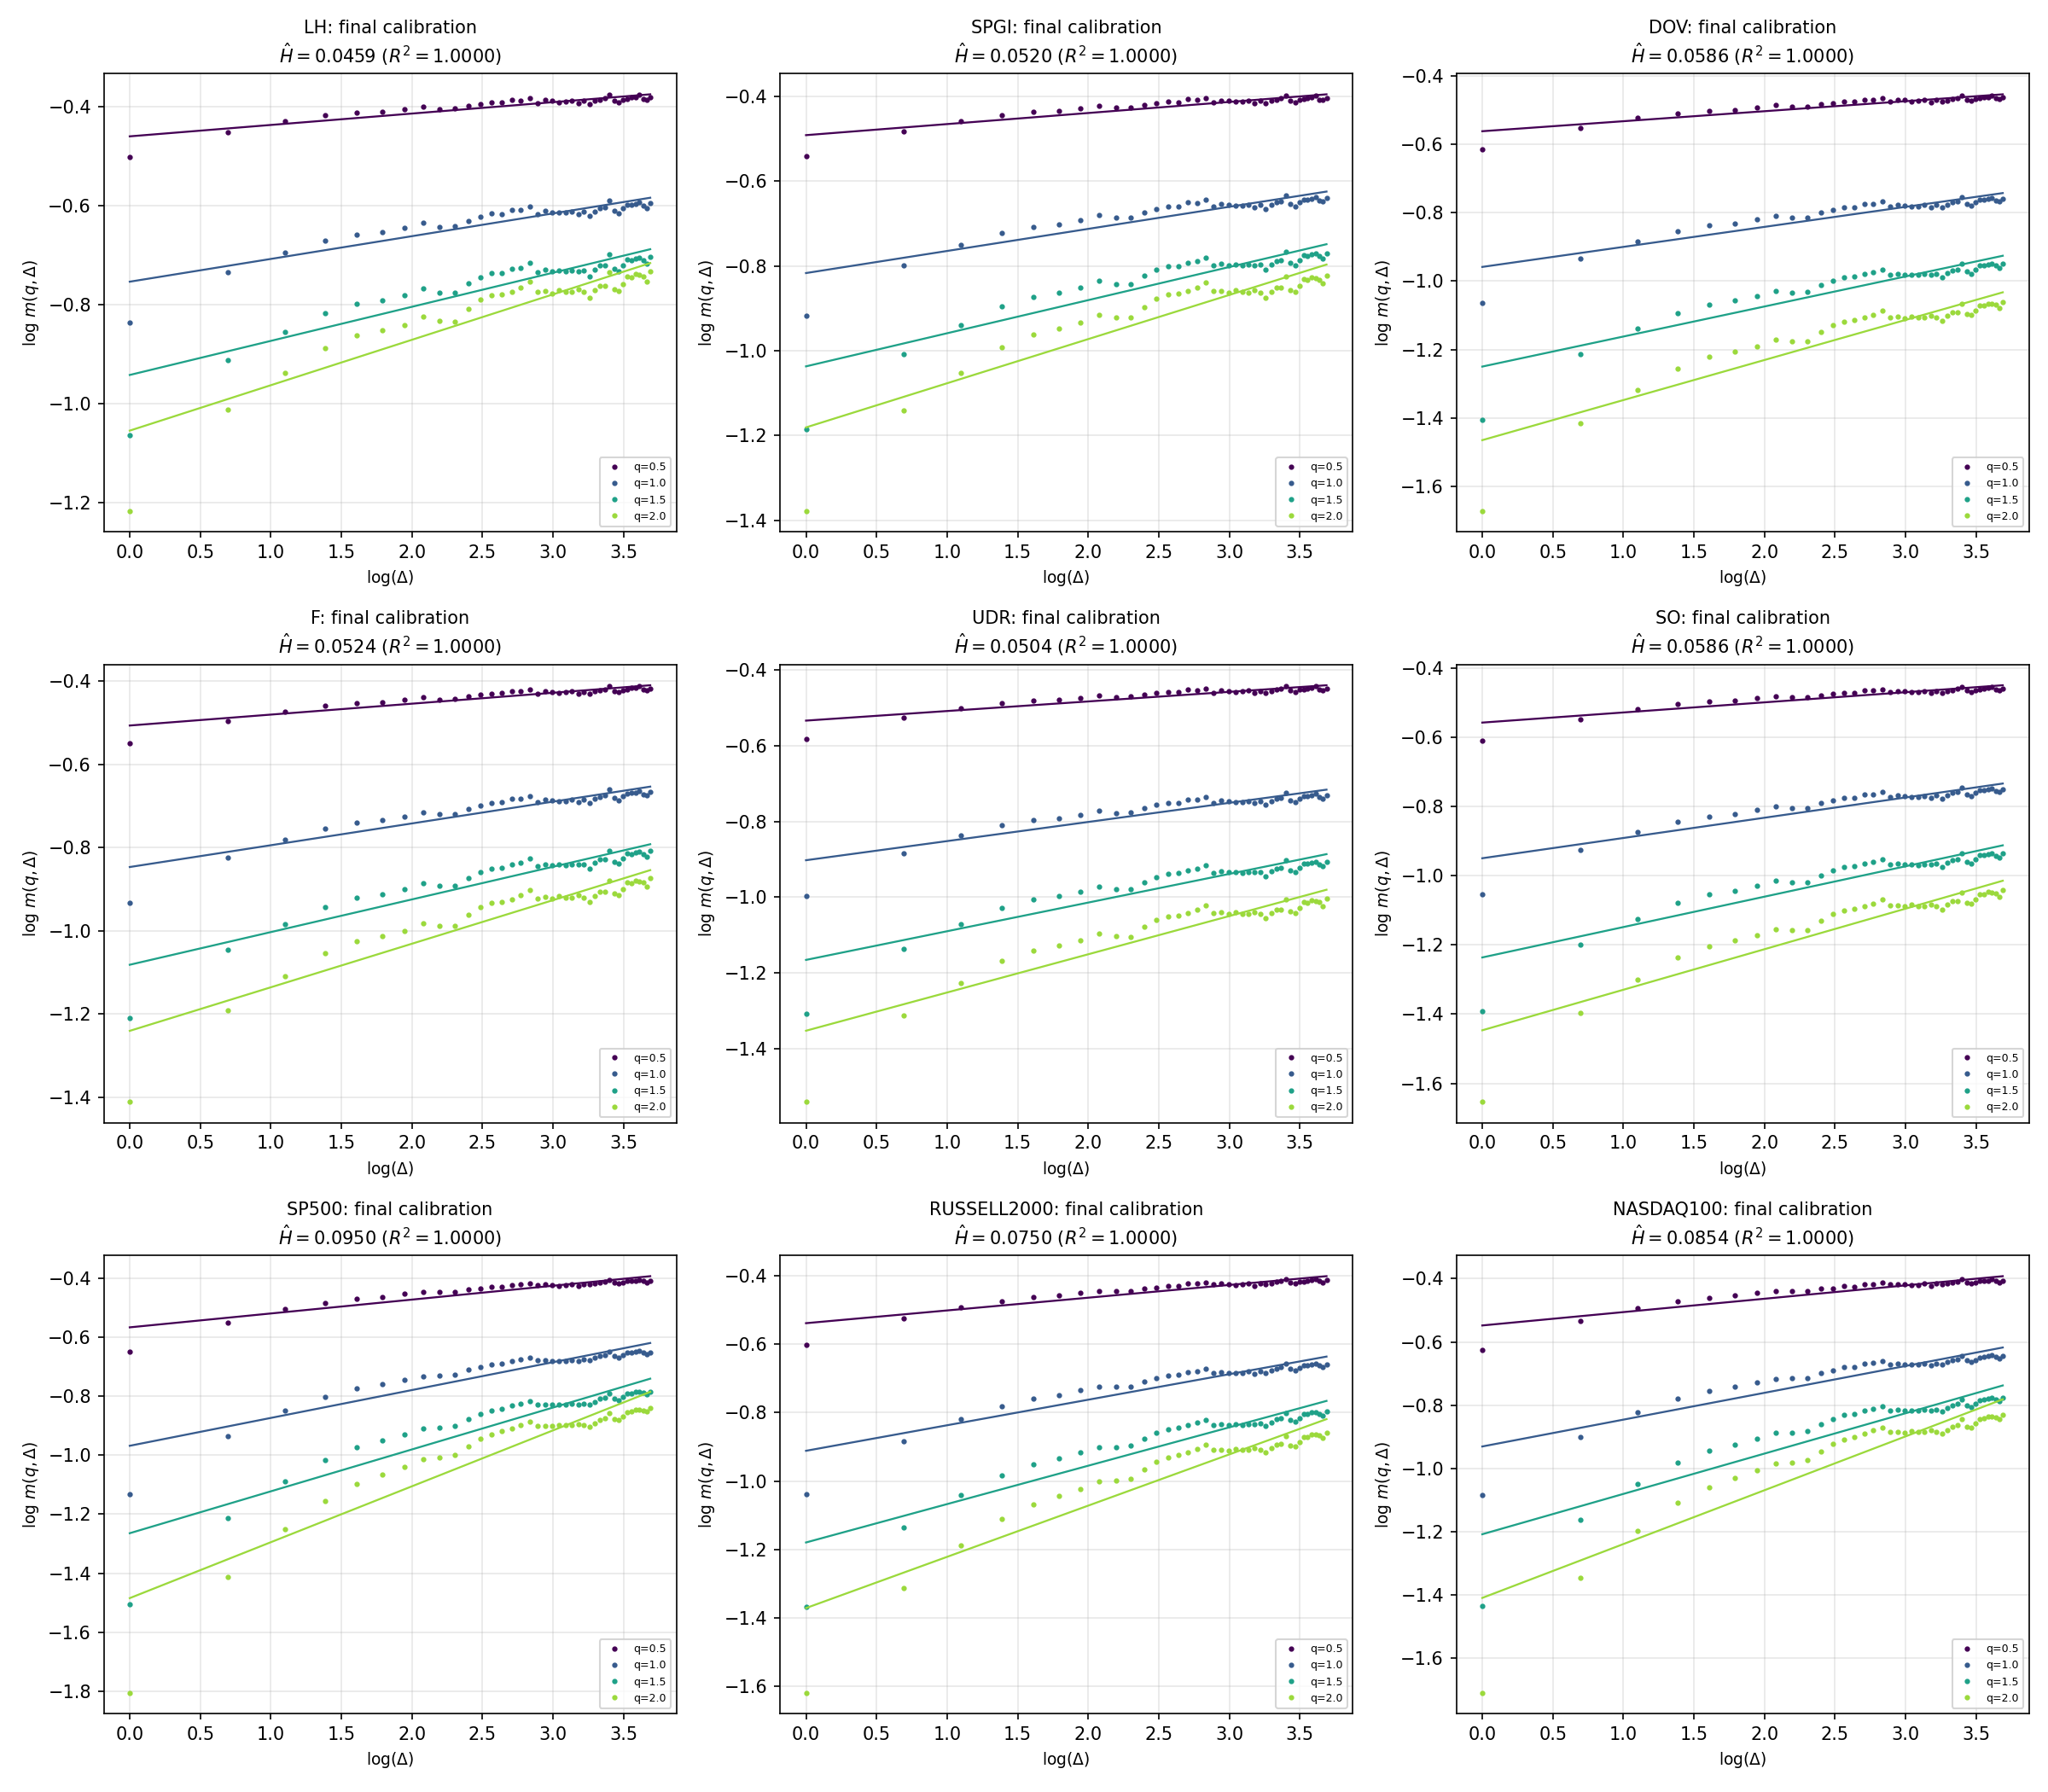
\includegraphics[width=0.98\textwidth]{logvol_moment_scaling_final_config.png}
\caption{Moment scaling curves $\log m(q,\Delta)$ vs.\ $\log\Delta$ for
$q\in\{0.5,1,1.5,2\}$, one panel per asset, each simulated at that asset's own
final calibrated $(H,\texttt{rough\_scale},\lambda_{lo},\lambda_{hi})$.}
\label{fig:momentscaling}
\end{figure}

\textbf{Every calibration gives an essentially perfect monofractal fit}
($R^2>0.999$ in every case shown) -- $\zeta(q)$ is close to exactly linear through
the origin at every asset's final calibrated point, confirming the simulated
log-volatility remains a genuinely rough, self-similar process throughout this
note's search space, not just near the companion note's own original centre
values.

\subsection{Interpretation}
\textbf{The 6 stocks and the 3 indices needed different regions of the same
4-parameter space to reach their own targets, and the calibration found both.}
Stocks' real log-volatility is rougher than what a companion-note-centred ESN
naturally produces; indices' is smoother. Freeing $\lambda_{lo},\lambda_{hi}$ gives
the calibration access to both directions from the same fixed architecture: for
stocks, calibrated $\lambda_{hi}$ stays close to the companion note's own centre
value ($3.0$--$3.9$); for indices, it drops substantially ($1.5$--$2.5$), consistent
with \S\ref{sec:calibexplain}'s mechanism (lower $\lambda_{hi}$ raises the
achievable roughness ceiling, which is what smoother, larger-$\hat H$ index targets
need relatively less of, and rougher stock targets need relatively more of the
companion note's own higher-$\lambda_{hi}$ regime to avoid overshooting past).
\texttt{SP500} needed the most extreme parameters of the 9 (the lowest
$\lambda_{hi}$, $1.50$, at the very edge of its bound) -- consistent with it having
the largest gap between its real roughness and the companion-note-centred
architecture's own achievable range of any asset examined across this whole note
family.

\section{Empirical distribution of the ESN's estimated Hurst exponent, vs.\ each asset's target}
\label{sec:empiricaldist}
\S\ref{sec:results}'s confirmation used a single, long ($T=8{,}000$-day) simulated
path per asset. This section asks how much that single-path estimate varies from
one simulated realisation to another, and whether each asset's real target sits
comfortably inside that variation: for each asset, \textbf{60 independent ESN
paths} are simulated at that asset's final calibrated
$(H,\texttt{rough\_scale},\lambda_{lo},\lambda_{hi})$, each $T=3{,}000$ days long,
and the same moment-scaling $\hat H$ is estimated separately on every path -- an
empirical distribution of 60 $\hat H$ values per asset.

\textbf{Definition of the $z$-score.} Writing $\bar H_{\text{ESN}}$ and
$\sigma_{\text{ESN}}$ for the empirical distribution's mean and standard deviation,
and $H_{\text{target}}$ for the asset's real, bias-corrected target,
\[
z = \frac{H_{\text{target}} - \bar H_{\text{ESN}}}{\sigma_{\text{ESN}}}\, ,
\]
the number of empirical standard deviations the real target sits away from the
ESN's typical simulated value -- $z=0$ means the target equals the empirical mean
exactly; $|z|$ larger than about $2$ would mean the target is an unusual draw from
the ESN's own distribution (roughly the top or bottom $5\%$, under a normal
approximation).

\begin{figure}[h]
\centering
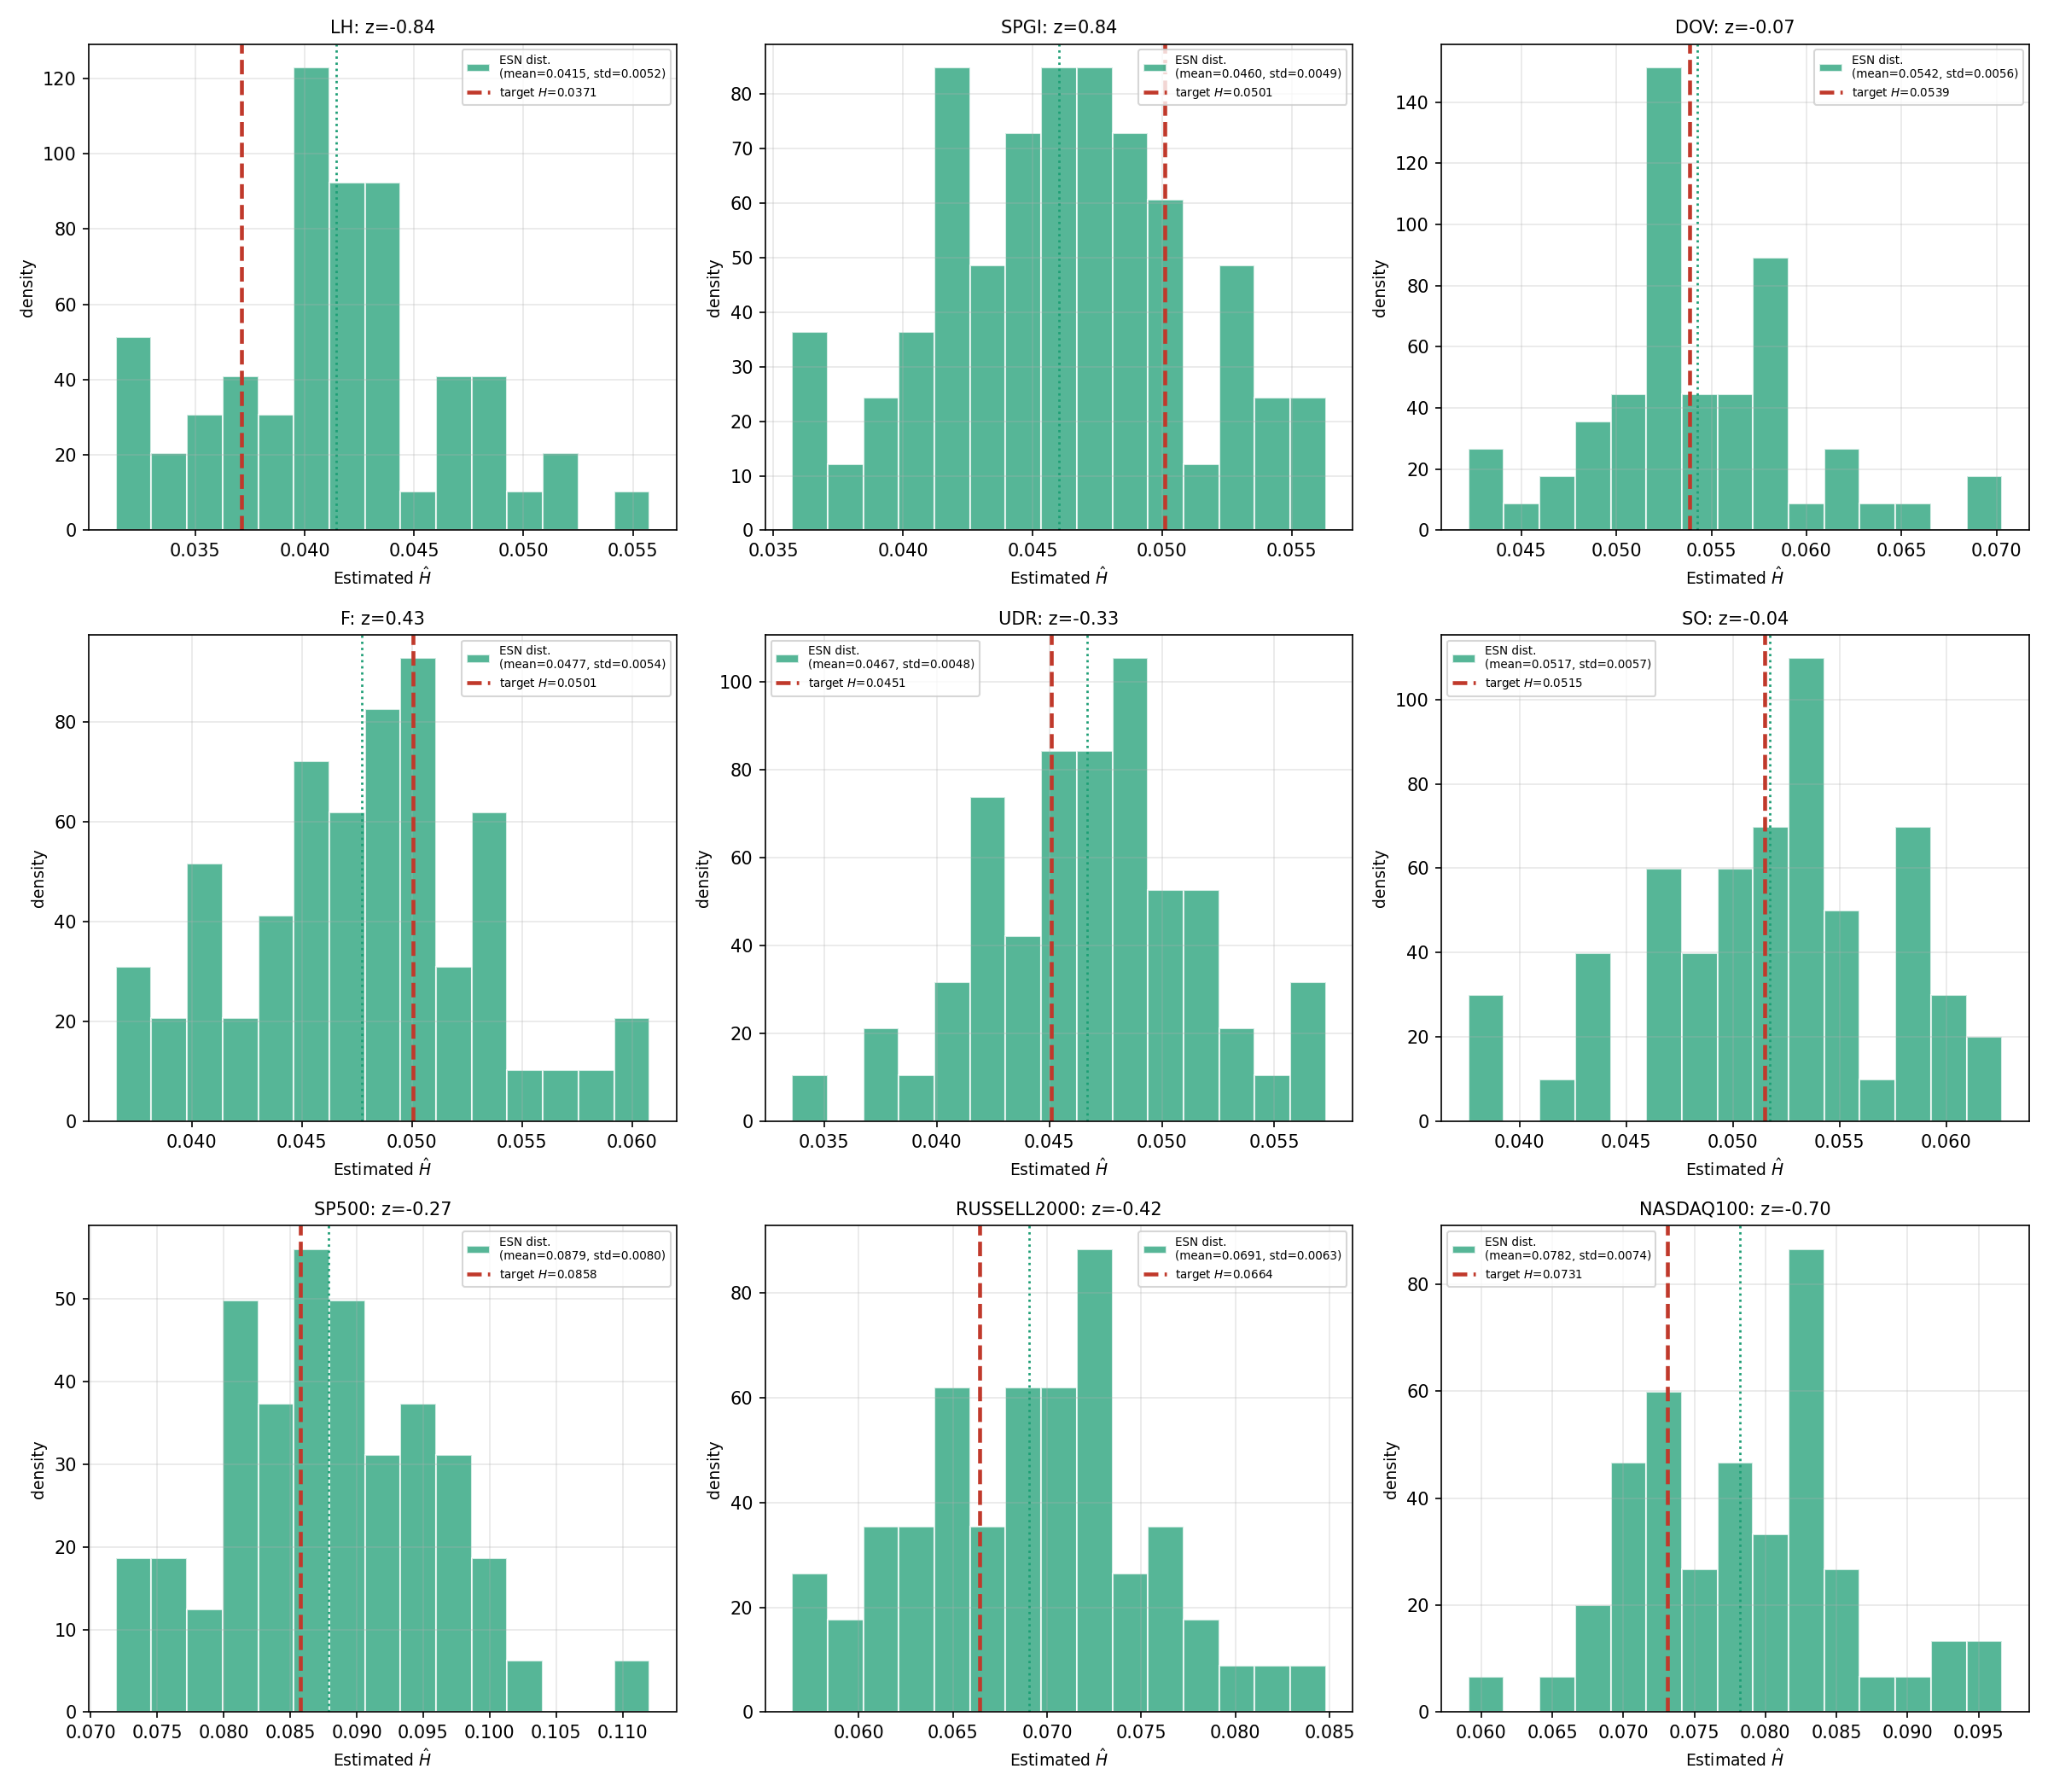
\includegraphics[width=0.98\textwidth]{esn_H_empirical_distribution_final_config.png}
\caption{Empirical distribution of the ESN's moment-based $\hat H$ (60 replicate
$T=3{,}000$-day paths), one panel per asset, vs.\ that asset's real, bias-corrected
target $H$ (dashed red line).}
\label{fig:empiricaldist}
\end{figure}

\begin{table}[h]
\centering
\caption{Empirical distribution summary and $z$-score, all 9 assets.}
\label{tab:zscores}
\begin{tabular}{lcccc}
\toprule
Asset & ESN $\hat H$ mean (std) & target $\hat H$ & $z$-score \\
\midrule
\texttt{LH}          & $0.0415$ $(0.0052)$ & $0.0371$ & $-0.84$ \\
\texttt{SPGI}        & $0.0460$ $(0.0049)$ & $0.0501$ & $+0.84$ \\
\texttt{DOV}         & $0.0542$ $(0.0056)$ & $0.0539$ & $-0.07$ \\
\texttt{F}           & $0.0477$ $(0.0054)$ & $0.0501$ & $+0.43$ \\
\texttt{UDR}         & $0.0467$ $(0.0048)$ & $0.0451$ & $-0.33$ \\
\texttt{SO}          & $0.0517$ $(0.0057)$ & $0.0515$ & $-0.04$ \\
\texttt{SP500}       & $0.0879$ $(0.0080)$ & $0.0858$ & $-0.27$ \\
\texttt{RUSSELL2000} & $0.0691$ $(0.0063)$ & $0.0664$ & $-0.42$ \\
\texttt{NASDAQ100}   & $0.0782$ $(0.0074)$ & $0.0731$ & $-0.70$ \\
\bottomrule
\end{tabular}
\end{table}

\textbf{Every one of the 9 assets has $|z|<1$} -- the largest are \texttt{LH}'s
$-0.84$ and \texttt{SPGI}'s $+0.84$, and the mean $|z|$ across all 9 is $0.44$.
\texttt{DOV} and \texttt{SO} are essentially exact ($|z|<0.1$). \textbf{This holds
for both directions of mismatch this note has found}: the 6 stocks, whose real
roughness exceeds a companion-note-centred ESN's own, and the 3 indices, whose real
roughness falls short of it. \textbf{The same fixed architecture, with only $H$,
\texttt{rough\_scale}, $\lambda_{lo}$, and $\lambda_{hi}$ free, reproduces the
moment-based Hurst exponent of every individual stock and every market index
examined in this note}, simultaneously, once calibrated directly to that target
with an adequately robust (multi-path, multi-start) optimisation.

\section{Limitations and Recommended Next Steps}
\label{sec:limitations}
\begin{enumerate}
\item \textbf{Only the 4 roughness-related entries of $p$ were calibrated; the
other 8 were held fixed at the grid-midpoint values described in
\S\ref{sec:pfixed} -- never individually optimised for roughness or any other
stylised fact.} Whether freeing more of $p$ (in particular the $z$-bank's own
rate range $a_{lo},a_{hi}$ and readout profile \texttt{zr\_lo},\texttt{zr\_hi})
would allow an even tighter roughness match, or would trade off against it the
way $\lambda_{lo},\lambda_{hi}$ initially did against the companion note's
aggregate score, was not tested.
\item \textbf{This calibration targets roughness exclusively}; the other 10
stylised facts (mean volatility, tail behaviour, volatility clustering, leverage,
kurtosis, etc.) are not tracked or optimised at all in this note's final
methodology. Whether the resulting $(H,\texttt{rough\_scale},\lambda_{lo},
\lambda_{hi})$ points also give a reasonable match on those other terms, or badly
sacrifice them for a precise roughness match, was not checked.
\item \textbf{The optimisation used up to 3 starting points and up to 12 paths per
evaluation}, chosen adaptively per asset as needed to reach $|z|<1$; a fixed,
uniform budget across all 9 assets from the outset was not used, so the exact
compute cost needed for a new, as-yet-uncalibrated asset is not precisely known in
advance.
\item \textbf{The single-path $T=8{,}000$-day confirmation used during calibration
is itself an imperfect proxy for the 60-replicate empirical mean}: for
\texttt{NASDAQ100} specifically, an early candidate's confirmation gap looked
better than its eventual empirical $z$-score turned out to be, and the discrepancy
was only caught by checking a partial replicate sample directly. Relying on the
empirical distribution (or a partial version of it) throughout calibration, rather
than only at the final check, may be more reliable, and was not adopted uniformly
across all 9 assets here.
\item \textbf{The 9 assets were not chosen for any particular economic or
sectoral reason} -- 3 continue the companion note's own selection permutation, 3
are independently randomly selected, and 3 indices were chosen as commonly-tracked
U.S.\ benchmarks. Whether this methodology generalises to other individual stocks,
other indices, or non-U.S.\ markets was not tested.
\end{enumerate}

\end{document}
